\documentclass[10pt]{article}
\usepackage[utf8]{inputenc}
\usepackage[T1]{fontenc}
\usepackage{amsmath}
\usepackage{amsfonts}
\usepackage{amssymb}
\usepackage[version=4]{mhchem}
\usepackage{stmaryrd}
\usepackage{graphicx}
\usepackage[export]{adjustbox}
\graphicspath{ {./images/} }
\usepackage{bbold}

\title{Probability and Statistics - Elementary Probability Theory }

\author{Giuliano Casale\\
Department of Computing, Imperial College London}
\date{}


\begin{document}
\maketitle


\section*{Discrete Random Variables}
We say a random variable is discrete if it can take only a countable number of possible values. That is,\\
$X$ is discrete $\Longleftrightarrow \operatorname{supp}(X)$ is countable.

Thus, $\operatorname{supp}(X)$ can either be finite or countably infinite.

\begin{itemize}
  \item Suppose $X$ is discrete, and can take values in the countable set $\operatorname{supp}(X)=\left\{x_{1}, x_{2}, \ldots\right\}$ ordered so that $x_{1}<x_{2}<\ldots$.
  \item The subset $S_{x}=\{s \in S \mid X(s) \leq x\}$ is thus constant as we increase $x$ in an interval $\left[x_{i-1}, x_{i}\right)$. Only once we reach $x=x_{i}$, $S_{x}$ grows larger to include the outcomes that map to $x_{i}$.
  \item Thus, $F_{X}$ will be a monotonic increasing step function with vertical jumps at points in $\operatorname{supp}(X)$, i.e.,
\end{itemize}

$$
F_{X}\left(x_{i}\right)=F_{X}\left(x_{i-1}\right)+\mathrm{P}_{X}\left(X=x_{i}\right)
$$

\begin{itemize}
  \item Equivalently, this may be re-written as
\end{itemize}

$$
\mathrm{P}_{X}\left(X=x_{i}\right)=F_{X}\left(x_{i}\right)-F_{X}\left(x_{i-1}\right)
$$

\section*{Example: Poisson(5) cdf}
The Poisson random variable with parameter 5 (defined later) has cdf that looks like this:\\
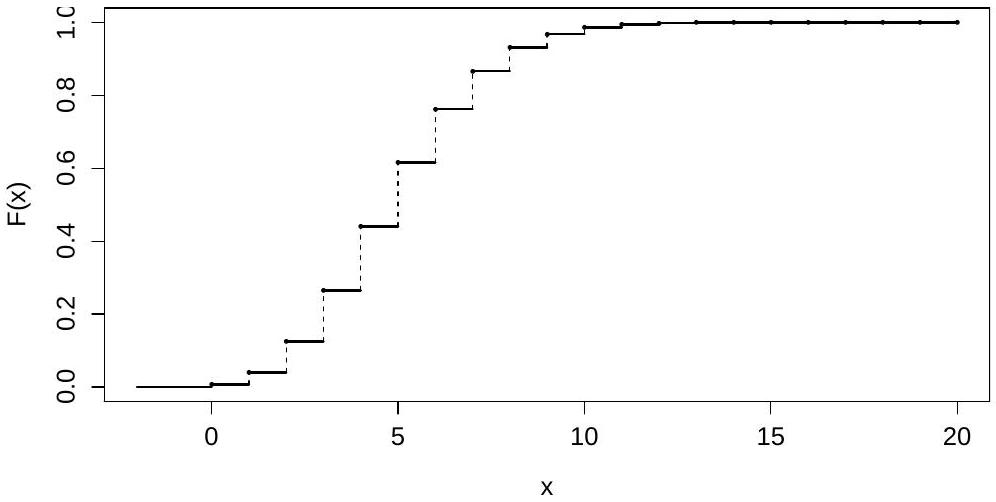
\includegraphics[max width=\textwidth, center]{2025_05_11_35704811148ad612caa6g-04}

\section*{Probability Mass Function}
For a discrete random variable $X$ and $x \in \mathbb{R}$, we define the probability mass function (pmf), $p(x)$ (more precisely $p_{X}(x)$ ) as

$$
p(x)=\mathrm{P}_{x}(X=x)
$$

If $X$ can take values $\operatorname{supp}(X)=\left\{x_{1}, x_{2}, \ldots\right\}$, then:\\
(1) $0 \leq p(x) \leq 1, \forall x \in \mathbb{R}$;\\
(2) $\sum_{x \in \operatorname{supp}(X)} p(x)=1$.

\section*{Example: Poisson(5) pmf}
The Poisson random variable with parameter 5 has pmf with a discrete plot that looks like:\\
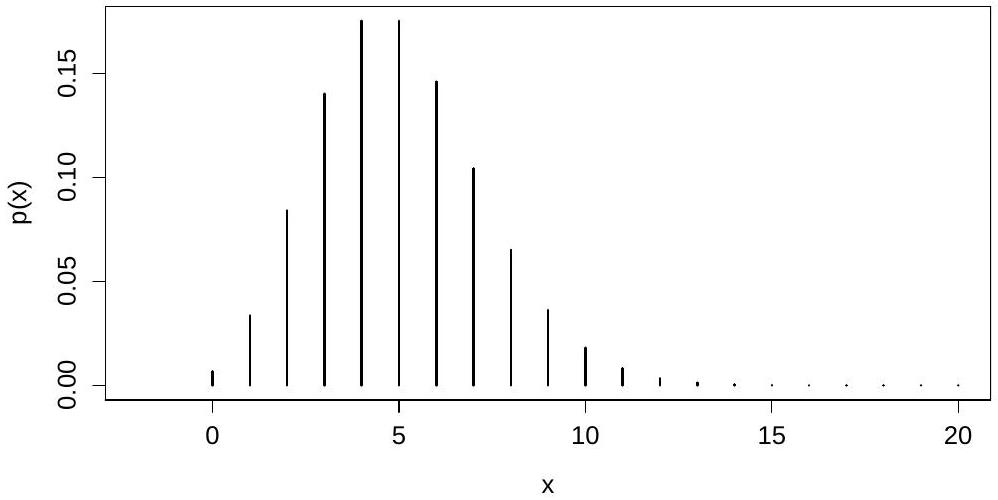
\includegraphics[max width=\textwidth, center]{2025_05_11_35704811148ad612caa6g-06}

\begin{itemize}
  \item Either the pmf or cdf of a discrete random variable fully characterises its probability distribution.
  \item Indeed, from the cdf we can derive the pmf, and vice versa since
\end{itemize}

$$
\begin{aligned}
& p\left(x_{i}\right)=F\left(x_{i}\right)-F\left(x_{i-1}\right), \\
& F\left(x_{i}\right)=\sum_{j=1}^{i} p\left(x_{j}\right) .
\end{aligned}
$$

\section*{Expectation}
\section*{Expectation: $\mathrm{E}[X]$}
For a discrete random variable $X$ we define the expectation of

\section*{Definition}
$$
E(X)=\sum_{x} x p(x)
$$

\begin{itemize}
  \item $\mathrm{E}(X)$ (often more precisely $\mathrm{E}_{X}(X)$ or even $\mu_{X}$ ) is also referred to as the mean of the distribution of $X$.
  \item $\mathrm{E}(X)$ gives a weighted average of the possible values of the random variable $X$, with the weights given by the probability of that particular outcome.
\end{itemize}

\section*{Examples}
(1) If $X$ is a r.v. taking the integer value scored with a single roll of a fair die, then

$$
\begin{aligned}
E(X) & =\sum_{x=1}^{6} x p(x) \\
& =1 \cdot \frac{1}{6}+2 \cdot \frac{1}{6}+3 \cdot \frac{1}{6}+4 \cdot \frac{1}{6}+5 \cdot \frac{1}{6}+6 \cdot \frac{1}{6}=\frac{21}{6}=3.5 .
\end{aligned}
$$

(2) Q: A student gets $X$ marks answering a single multiple choice question with four options, where 3 marks are awarded for a correct answer and -1 for a wrong answer. What is the expected value for a random answer?

\section*{Expectation of a function of a random variable: $\mathrm{E}(g(X))$}
More generally, for a (measurable) function of interest $g: \mathbb{R} \rightarrow \mathbb{R}$ of the random variable $X$, we notice that $g(X)$,

$$
g(X)(s)=(g \circ X)(s)
$$

is also a random variable, where o denotes composition. It then follows that


\begin{equation*}
\mathrm{E}(g(X))=\sum_{x} g(x) p(x) \tag{1}
\end{equation*}


\section*{Linearity of Expectation}
Consider the linear function $g(X)=a X+b$ for constants $a, b \in \mathbb{R}$.

\begin{itemize}
  \item We can see from (1) that
\end{itemize}

$$
\begin{aligned}
\mathrm{E}(a X+b) & =\sum_{x}(a x+b) p(x) \\
& =a \sum_{x} x p(x)+b \sum_{x} p(x)
\end{aligned}
$$

\begin{itemize}
  \item since $\sum_{x} x p(x)=\mathrm{E}(X)$ and $\sum_{x} p(x)=1$ we have
\end{itemize}

$$
\mathrm{E}(a X+b)=a \mathrm{E}(X)+b, \quad \forall a, b \in \mathbb{R} .
$$

It is equally easy to check that for $g, h: \mathbb{R} \rightarrow \mathbb{R}$, we have

$$
\mathrm{E}(g(X)+h(X))=\mathrm{E}(g(X))+\mathrm{E}(h(X)) .
$$

Moments

\section*{Variance: $\operatorname{Var}(X)$}
The expectation of a function $g(X)=X^{n}$ gives us the $n^{\text {th }}$ (raw) moment of $X$.

A central moment is similarly defined, but re-centered to characterize the deviation from the mean. Choose for example:

$$
g(X)=(X-\mathrm{E}(X))^{2} .
$$

The expectation of this function with respect to $P_{X}$ gives a measure of the variability of the r.v. $X$ around its mean, called the variance and denoted $\operatorname{Var}(X)$ (or $\operatorname{Var}_{X}(X)$ or sometimes $\sigma_{X}^{2}$ ).

\section*{Definition}
$$
\operatorname{Var}(X)=\mathrm{E}\left[(X-\mathrm{E}(X))^{2}\right] .
$$

We can expand the expression $(X-\mathrm{E}(X))^{2}$ and use the linearity of expectation to get an alternative formula for the variance:

$$
\begin{aligned}
(X-\mathrm{E}(X))^{2} & =X^{2}-2 \mathrm{E}(X) X+(\mathrm{E}(X))^{2} \\
\Rightarrow \operatorname{Var}(X) & =\mathrm{E}\left[X^{2}-(2 \mathrm{E}(X)) X+(\mathrm{E}(X))^{2}\right] \\
& =\mathrm{E}\left(X^{2}\right)-2 \mathrm{E}(X) \mathrm{E}(X)+(\mathrm{E}(X))^{2}
\end{aligned}
$$

and hence

$$
\operatorname{Var}(X)=\mathrm{E}\left(X^{2}\right)-(\mathrm{E}(X))^{2} .
$$

\section*{Variance of a Linear Function of a Random Variable}
\begin{itemize}
  \item Corresponding to the linearity of expectation, i.e. $\mathrm{E}(a X+b)=a \mathrm{E}(X)+b$ for constants $a, b \in \mathbb{R}$, for variance we have:
\end{itemize}

$$
\operatorname{Var}(a X+b)=a^{2} \operatorname{Var}(X), \quad \forall a, b \in \mathbb{R} .
$$

\begin{itemize}
  \item Proof follows by expanding the definition of Var (left as an exercise).
\end{itemize}

\section*{Standard deviation: $\operatorname{sd}(X)$}
The standard deviation of a random variable $X$, written $\operatorname{sd}(X)$ (or sometimes $\sigma_{X}$ ), is the square root of the variance:

\section*{Definition}
$$
\operatorname{sd}(X)=\sqrt{\operatorname{Var}_{X}(X)}
$$

\section*{Examples}
(1) If $X$ is a r.v. taking the integer value scored with a single roll of a fair die, then

$$
\begin{aligned}
\operatorname{Var}(X) & =\sum_{x=1}^{6} x^{2} p(x)-3.5^{2} \\
& =1^{2} \cdot \frac{1}{6}+2^{2} \cdot \frac{1}{6}+\ldots+6^{2} \cdot \frac{1}{6}-(7 / 2)^{2}=35 / 12 .
\end{aligned}
$$

(2) Q: If $Y$ is a student's mark on a multiple choice question with four options, with 3 marks for a correct answer and -1 for a wrong answer, what is the standard deviation of a random choice?

\section*{Skewness}
\begin{itemize}
  \item The skewness $\left(\gamma_{1}\right)$ of a discrete random variable $X$, is a measure of its asymmetry. It is expressed as the following standardized moment:
\end{itemize}

\section*{Definition}
$$
\gamma_{1}=\frac{\mathrm{E}\left[(X-\mathrm{E}(X))^{3}\right]}{\operatorname{sd}(X)^{3}} .
$$

\begin{itemize}
  \item Commonly we have $\mu=\mathrm{E}(X)$ and $\sigma=\operatorname{sd}(X)$, and then we can write:
\end{itemize}

$$
\gamma_{1}=\frac{\mathrm{E}\left[(X-\mu)^{3}\right]}{\sigma^{3}} .
$$

\section*{Skew of a distribution}
The skewness helps to capture the asymmetry of the distribution:\\
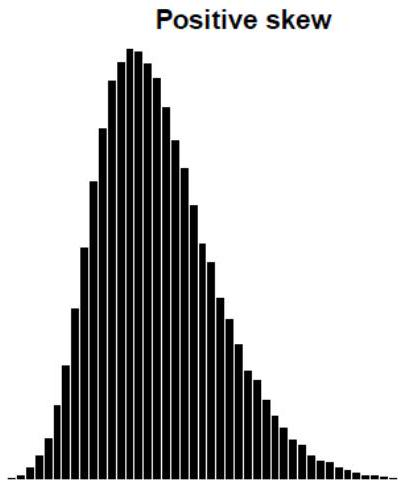
\includegraphics[max width=\textwidth, center]{2025_05_11_35704811148ad612caa6g-20(1)}\\
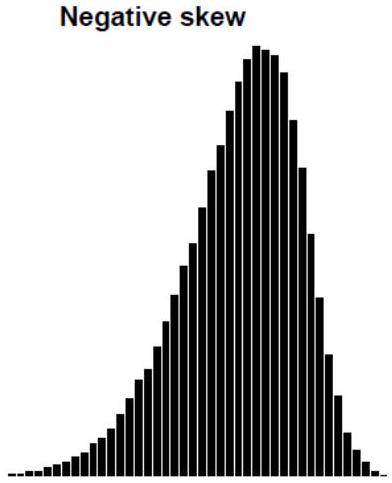
\includegraphics[max width=\textwidth, center]{2025_05_11_35704811148ad612caa6g-20}

\section*{Sum of Random Variables}
\section*{Motivating example}
Consider the following game: we flip a fair coin $n$ times and win $\pounds 1$ every time we get heads and $\pounds 0$ otherwise. What is the expected amount of money $S_{n}$ that we are going to win?

Calling $X_{i} \in\{0,1\}$ the random variable that models the outcome of the $i$-th toss, where $X_{i}(\{H\})=1$ and $X_{i}(\{T\})=0$, the amount we win is the random variable

$$
S_{n}=X_{1}+X_{2}+\ldots+X_{n}
$$

Our problem is therefore to quantify $E\left[S_{n}\right]$. Intuitively, since the repetitions are independent and the coin is fair, we expect to win half of the times, i.e., $E\left[S_{n}\right]=n / 2$. How do we formalize this?

\section*{Expectation of a Sum of Random Variables}
Let $X_{1}, X_{2}, \ldots, X_{n}$ be $n$ random variables, possibly with different distributions and not necessarily independent.

Let $S_{n}=\sum_{i=1}^{n} X_{i}$ be their sum, and $\bar{X}=\frac{S_{n}}{n}$ be their average.\\
Then:

$$
\mathrm{E}\left(S_{n}\right)=\sum_{i=1}^{n} \mathrm{E}\left(X_{i}\right), \quad \mathrm{E}(\bar{X})=\frac{\sum_{i=1}^{n} \mathrm{E}\left(X_{i}\right)}{n} .
$$

We will give a proof when we consider joint random variables.

\section*{Variance of a Sum of Independent Random Variables}
If the random variables $X_{1}, X_{2}, \ldots, X_{n}$ are independent, then:

$$
\operatorname{Var}\left(S_{n}\right)=\sum_{i=1}^{n} \operatorname{Var}\left(X_{i}\right), \quad \operatorname{Var}(\bar{X})=\frac{\sum_{i=1}^{n} \operatorname{Var}\left(X_{i}\right)}{n^{2}}
$$

So if $X_{1}, X_{2}, \ldots, X_{n}$ are independent and identically distributed (i.i.d.) with $\mathrm{E}\left(X_{i}\right)=\mu_{X}$ and $\operatorname{Var}\left(X_{i}\right)=\sigma_{X}^{2}$ we get

$$
E(\bar{X})=\mu_{X}, \quad \operatorname{Var}(\bar{X})=\frac{\sigma_{X}^{2}}{n} .
$$

\section*{Notable Discrete Distributions}
\section*{Bernoulli(p)}
\begin{itemize}
  \item Consider an experiment with only two possible outcomes, encoded as a random variable $X$ taking values 1 , with probability $p$; and 0 , with probability ( $1-p$ ).
  \item For example, tossing a coin with probability $p$ for heads: $X=1$ for heads; $X=0$ for tails.
  \item Then we say $X \sim \operatorname{Bernoulli}(p)$ and note the pmf to be
\end{itemize}

$$
p(x)=p^{x}(1-p)^{1-x}, \quad x=0,1 .
$$

\begin{itemize}
  \item Using the formulae for mean and variance, it follows that
\end{itemize}

$$
\mu=p, \quad \sigma^{2}=p(1-p) .
$$

\section*{Example: Bernoulli $\left(\frac{1}{4}\right)$ pmf}
\begin{center}
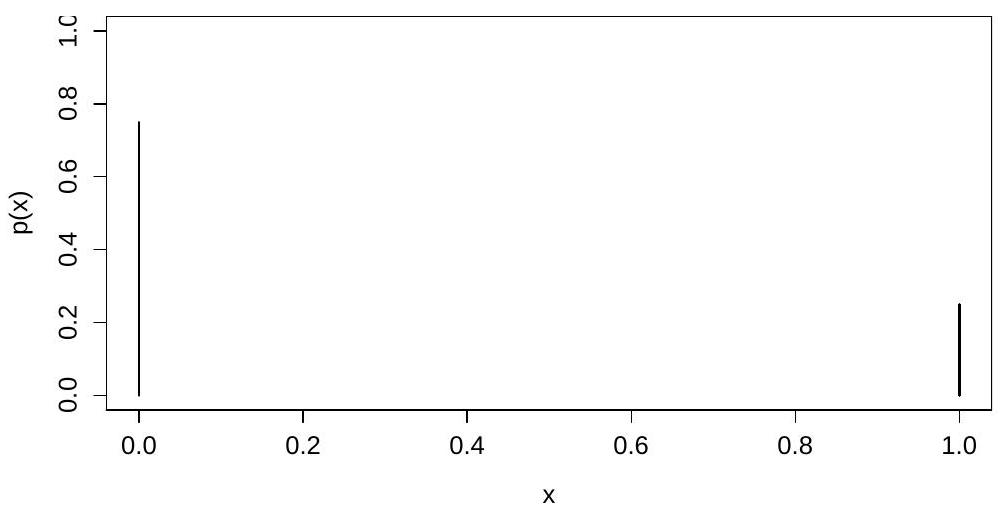
\includegraphics[max width=\textwidth]{2025_05_11_35704811148ad612caa6g-27}
\end{center}

\section*{$\operatorname{Binomial}(n, p)$}
\begin{itemize}
  \item Now consider $n$ identical, independent Bernoulli $(p)$ trials $X_{1}, \ldots, X_{n}$.
  \item Let $X=\sum_{i=1}^{n} X_{i}$ be the total number of 1 s observed in the $n$ trials.
  \item For example, tossing a fair coin $n$ times, $X$ may be the number of heads obtained, $p=\frac{1}{2}$.
  \item Then $X$ is a random variable taking values in $\{0,1,2, \ldots, n\}$, and we say $X \sim \operatorname{Binomial}(n, p)$.
  \item From the Binomial Theorem we find the pmf to be
\end{itemize}

$$
p(x)=\binom{n}{x} p^{x}(1-p)^{n-x}, \quad x=0,1,2, \ldots, n .
$$

\section*{Proof and moments}
\begin{itemize}
  \item Use simple combinatorial arguments, remembering that
\end{itemize}

$$
\binom{n}{x}=\frac{n!}{x!(n-x)!}
$$

\begin{itemize}
  \item Mean and variance are (from pmf or results on sums of r.vs.)
\end{itemize}

$$
\mu=n p, \quad \sigma^{2}=n p(1-p)
$$

\begin{itemize}
  \item Similarly, the skewness is:
\end{itemize}

$$
\gamma_{1}=\frac{1-2 p}{\sqrt{n p(1-p)}}
$$

\section*{Example: Binomial $\left(20, \frac{1}{4}\right)$ pmf}
\begin{center}
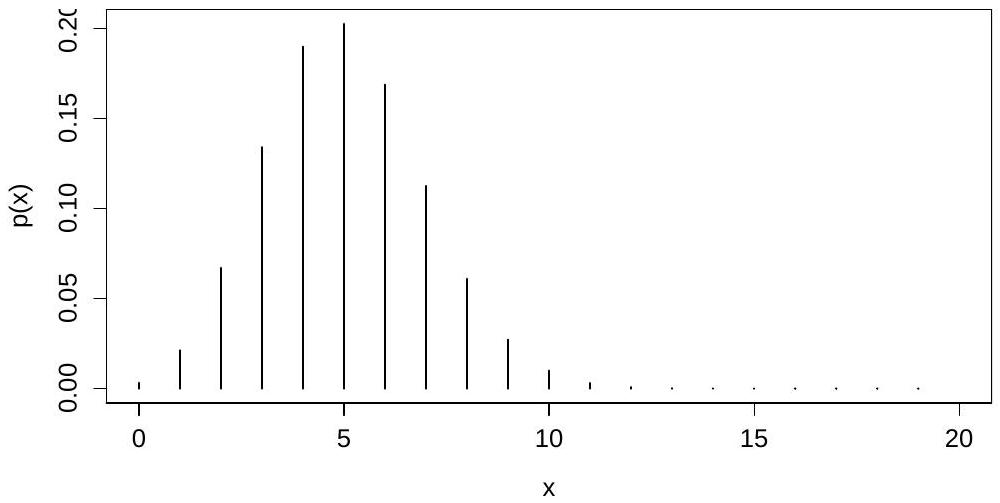
\includegraphics[max width=\textwidth]{2025_05_11_35704811148ad612caa6g-30}
\end{center}

\section*{Geometric(p)}
Consider a potentially infinite sequence of independent Bernoulli $(p)$ random variables $X_{1}, X_{2}, \ldots$.

\begin{itemize}
  \item Suppose we define a quantity $X$ by
\end{itemize}

$$
X=\min \left\{i \mid i \geq 1, X_{i}=1\right\}
$$

to be the index of the first Bernoulli trial to result in a 1 .

\begin{itemize}
  \item Then $X$ is a random variable taking values in $\operatorname{supp}(X)=\{1,2, \ldots\}$, and we say $X \sim \operatorname{Geometric}(p)$.
\end{itemize}

Example: Tossing a coin

\begin{itemize}
  \item $X$ is the number of tosses until the first head is obtained.
  \item The pmf is:
\end{itemize}

$$
p(x)=p(1-p)^{x-1}, \quad x=1,2, \ldots
$$

\begin{itemize}
  \item The mean and variance are:
\end{itemize}

$$
\mu=\frac{1}{p}, \quad \sigma^{2}=\frac{1-p}{p^{2}}
$$

\begin{itemize}
  \item The skewness is:
\end{itemize}

$$
\gamma_{1}=\frac{2-p}{\sqrt{1-p}}
$$

and so is always positive.\\
Remark: some texts call Geometric the distribution of the number of trials before we obtain our first 1 . Formulas for pmf and moments are similar.

\section*{Example: Geometric $\left(\frac{1}{4}\right)$ pmf}
\begin{center}
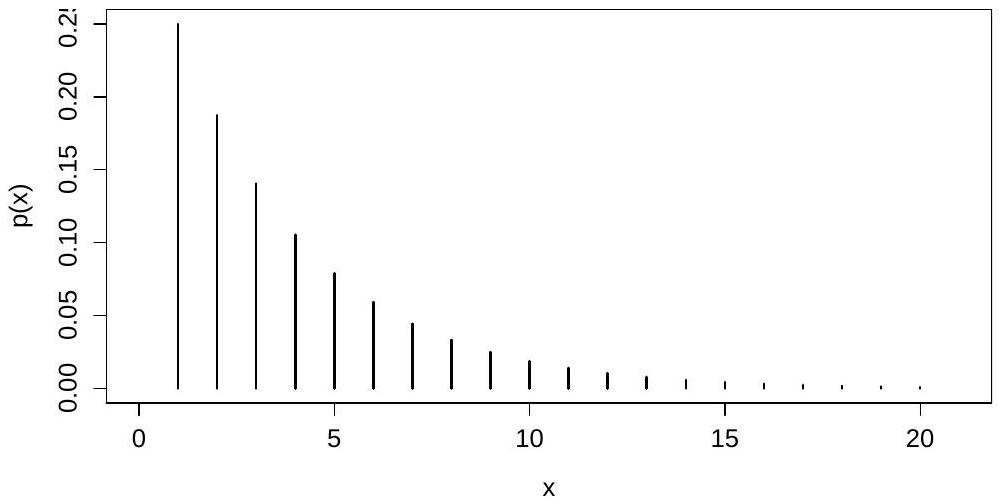
\includegraphics[max width=\textwidth]{2025_05_11_35704811148ad612caa6g-33}
\end{center}

\section*{Poisson: $\operatorname{Poi}(\lambda)$}
\begin{itemize}
  \item Let $X$ be a random variable on $\mathbb{N}=\{0,1,2, \ldots\}$. Define
\end{itemize}

$$
p(x)=\frac{e^{-\lambda} \lambda^{x}}{x!}, \quad x=0,1,2, \ldots
$$

for some $\lambda>0$.

\begin{itemize}
  \item Then, $X$ is said to follow a Poisson distribution with parameter $\lambda$ and we write $X \sim \operatorname{Poi}(\lambda)$.
  \item Poisson random variables are concerned with the number of random events occurring per unit of time or space, if there is a constant rate of random events occurring across this unit.
\end{itemize}

\section*{Examples}
\begin{itemize}
  \item the number of patients arriving at an emergency room in a hour;
  \item the number of minor car crashes per day in the U.K.;
  \item the number of potholes in each mile of road;
  \item the number of jobs which arrive at a database server per hour;
  \item the number of particles emitted by a radioactive substance in a given time.
  \item An interesting property of the Poisson distribution is that it has equal mean and variance, namely
\end{itemize}

$$
\mu=\lambda, \quad \sigma^{2}=\lambda
$$

\begin{itemize}
  \item The skewness is given by
\end{itemize}

$$
\gamma_{1}=\frac{1}{\sqrt{\lambda}}
$$

so is always positive but decreasing as $\lambda$ grows.

\section*{Example: Poi(5) pmf}
\begin{center}
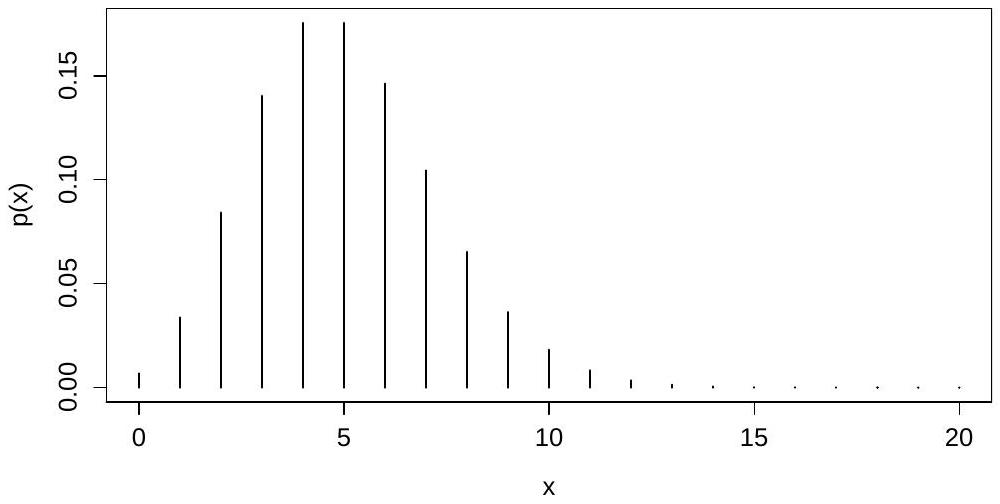
\includegraphics[max width=\textwidth]{2025_05_11_35704811148ad612caa6g-37}
\end{center}

\section*{Using the Poisson Distribution in practice}
\begin{itemize}
  \item What do we do if we have a non-unit interval (or space) of length $t$ ?
  \item In this case, $\lambda t$ can be used in the pmf instead of $\lambda$, so that
\end{itemize}

$$
p(x)=\frac{e^{-\lambda t}(\lambda t)^{x}}{x!}, \quad x=0,1,2, \ldots
$$

and we write $X \sim \operatorname{Poi}(\lambda t)$.

\begin{itemize}
  \item We thus now see $\lambda$ as the rate at which random events occur and $\lambda t$ as the mean number of events in $t$.
  \item Thus, both with $t=1$ and $t \neq 1$, we see the input parameter to the Poisson as the mean of the distribution.
\end{itemize}

\section*{Uniform: $\cup(\{1,2, \ldots, n\})$}
\begin{itemize}
  \item Let $X$ be a random variable on $\{1,2, \ldots, n\}$ with pmf
\end{itemize}

$$
p(x)=\frac{1}{n}, \quad x=1,2, \ldots, n .
$$

\begin{itemize}
  \item Then $X$ is said to follow a discrete uniform distribution and we write $X \sim \mathrm{U}(\{1,2, \ldots, n\})$.
  \item The mean and variance are
\end{itemize}

$$
\mu=\frac{n+1}{2}, \quad \sigma^{2}=\frac{n^{2}-1}{12} .
$$

\begin{itemize}
  \item Q: what value do you expect for the skewness?
\end{itemize}

\section*{Q\&A: Coupon collector problem}
\begin{center}

\includegraphics[max width=\textwidth]{2025_05_11_35704811148ad612caa6g-40}
\end{center}

A company producing cereals places 1 coupon in each cereal box. There are $m$ types of coupons and we wish to collect them all.

Suppose that each coupon type is equally-likely and independent of what has been previously obtained, i.e., the cereal boxes on the market are so many that drawing can be assumed with replacement.

Q: Find the mean number of boxes $X$ that we need to obtain in order to have at least one coupon of each type.


\end{document}